% This file was adapted from ICLR2022_conference.tex example provided for the ICLR conference
\documentclass{article} % For LaTeX2e
\usepackage{collas2023_conference,times}
\usepackage{easyReview}

% Please leave these options as they are
\usepackage{hyperref}
\hypersetup{
	colorlinks=true,
	linkcolor=red,
	filecolor=magenta,
	urlcolor=blue,
	citecolor=purple,
	pdftitle={Overleaf Example},
	pdfpagemode=FullScreen,
}



%
% These are recommended to typeset algorithms but not required. See the subsubsection on algorithms. Remove them if you don't have algorithms in your paper.
\usepackage{algorithm}
%\usepackage{algorithmic}


%
% Keep the \pdfinfo as shown here. There's no need
% for you to add the /Title and /Author tags.
\pdfinfo{
	/TemplateVersion (2023.3)
}


\setcounter{secnumdepth}{2}


\usepackage{amssymb}
\usepackage{amsthm}
\usepackage{amsmath}
\usepackage[noend]{algpseudocode}


\usepackage{multirow}
\usepackage{ctable}


\usepackage{caption, subcaption}


%%\usepackage[utf8]{inputenc} % allow utf-8 input
%\usepackage[T1]{fontenc}    % use 8-bit T1 fonts
%%\usepackage[backref=page]{hyperref}       % hyperlinks
%\usepackage{url}            % simple URL typesetting
\usepackage{booktabs}       % professional-quality tables
%\usepackage{amsfonts}       % blackboard math symbols
\usepackage{nicefrac}       % compact symbols for 1/2, etc.
%\usepackage{microtype}      % microtypography
%\usepackage{xcolor}         % colors

\theoremstyle{definition}
\newtheorem{defn}{Definition}[section]
\newtheorem{theorem}{Theorem}[section]
\newtheorem{proposition}[theorem]{Proposition}
\newtheorem{corollary}[theorem]{Corollary}
\newtheorem{lemma}[theorem]{Lemma}
\newtheorem{hypothesis}[theorem]{Hypothesis}
\newtheorem{assumption}[theorem]{Assumption}
\newcommand{\Expect}[2]{\mathbb{E}_{#1}\left [#2 \right ]}
\newcommand{\RM}[1]{\textcolor{magenta}{\{RM: #1\}}}
\newcommand{\LF}[1]{\textcolor{blue}{\{LF: #1\}}}
\newcommand{\LFe}[1]{\textcolor{blue}{#1}}

\usepackage[utf8]{inputenc}

% Your title must be in mixed case, not sentence case.
% That means all verbs (including short verbs like be, is, using,and go),
% nouns, adverbs, adjectives should be capitalized, including both words in hyphenated terms, while
% articles, conjunctions, and prepositions are lower case unless they
% directly follow a colon or long dash
\title{Adaptive Meta-Learning via data-dependent PAC-Bayes bounds}
\author{
	%Authors
	% All authors must be in the same font size and format.
	Lior Friedman,\textsuperscript{\rm 1}
	Ron Meir\textsuperscript{\rm 1}
}

%\affiliations{
	%Afiliations
%	\textsuperscript{\rm 1} 
%	The Viterbi Faculty of Electrical and Computer Engineering\\
%	Technion - Israel Institute of Technology\\
%	Haifa 3200003, Israel\\
%	liorf@campus.technion.ac.il, rmeir@ee.technion.ac.il
%}

\begin{document}
	
\maketitle

\begin{abstract}
	Meta-learning aims to extract common knowledge from similar training tasks in order to facilitate efficient and effective learning on future tasks. Several recent works have extended PAC-Bayes generalization error bounds to the meta-learning setting.
	By doing so, prior knowledge can be incorporated in the form of a distribution over hypotheses that is expected to lead to low error on new tasks that are similar to those that have been previously observed.
	In this work, we develop novel bounds for the generalization error on test tasks based on recent data-dependent bounds and provide a novel algorithm for adapting prior knowledge to downstream tasks in a potentially more effective manner.
	We demonstrate the effectiveness of our algorithm numerically for few-shot image classification tasks with deep neural networks and show a significant reduction in generalization error without any additional adaptation data.
\end{abstract}

\section{Introduction}

% ml, meta-learning and few-shot
Over the last few decades, the field of machine learning has developed rapidly both theoretically and as an engineering practice. Of particular interest is the field of learning and adapting quickly from only a few examples, which requires a balance between prior experience and new information in order to solve new tasks effectively without overfitting.
One common approach to tackle this few-shot learning problem is that of meta-learning, where training data is used to create a prior that is conducive to the downstream task. This approach has shown promising empirical results in a variety of domains (see survey \citep{Hospedales2021}), especially for cases with few test examples.

As an illustrative example of the meta-learning problem, we might consider a visual classification system that must also be capable of identifying new categories of objects with very few examples. In order to achieve this goal, the system must maintain prior knowledge on similar vision problems, and utilize this prior to adapt quickly to the new data.

In order to better understand the generalization capabilities of classification methods and give upper bounds on the gap between the training and test performance, several theoretical frameworks have been devised.  Among these frameworks, methods based on PAC-Bayes bounds \citep{Mcallester} are of particular interest, as they result in practical optimization algorithms with potentially non-vacuous generalization guarantees with high probability. As such, it is not surprising that several works have extended the PAC-Bayes framework to the domain of meta-learning, such as \citet{Pentina2014}, \citet{Amit2018}, \citet{Rothfuss2020}, \citet{Liu2021} and \citet{Farid2021}.

Several recent works have established non-vacuous generalization bounds for practical deep learning problems, such as the methods suggested by \citet{Dziugaite2017} and later improved by \citet{Perez-Ortiz2021}. In both cases, the use of a \emph{data-dependent} prior was shown to be a major component in achieving these impressive results. As such, data-dependent PAC-Bayes bounds such as those proposed in \citet{Rivasplata2020} may be of great interest for meta-learning.

In this work, we utilize data-dependent PAC-Bayes techniques to provide an upper bound on the generalization error for new tasks by adapting an existing distribution over priors to better fit the given test task. This approach allows us to use existing methods to meta-learn a distribution over training tasks and provides a potentially tighter guarantee for the new task.
We compare our bounds to known bounds for a simple setting, and develop a practical algorithm based on our bounds. We demonstrate the effectiveness of this meta-adaptation approach for classification on vision tasks.

\section{Background}

\subsection{PAC-Bayes bounds}

The common setting for learning consists of a set of independent examples $S=\{z_i\}_{i=1}^{m}\subset \mathcal{Z}^m$, drawn from an unknown distribution $z_i\sim \mathcal{D}$. We denote $S\sim \mathcal{D}^m$ the distribution over the samples. 
For the common setting of classification, each example $z_i=(x_i,y_i)$ is a pair of data and label.
Given a space of hypotheses $\mathcal{H}$ and a sample $S$, we would like to find a hypothesis $h\in \mathcal{H}$ that minimizes the \emph{expected loss} $\Expect{z\sim \mathcal{D}}{\ell(h,z)}$, where $\ell:\mathcal{Z}\rightarrow [a,b]$ is a bounded loss function (some PAC-Bayes bounds apply for unbounded losses with concentration properties such as sub-gamma and sub-Gaussian distributions, and may be useful for future extensions).
Since $\mathcal{D}$ is unknown, we must use the training data $S$ to find a hypothesis that minimizes the expected loss with high probability, based on the sample of size $m$.%\RM{Think where we want to refer to bounded versus unbounded loss}

The PAC-Bayes framework, as formulated by \citet{Mcallester}, takes as input the training data $S$ as well as an inductive bias in the form of a prior distribution $P$ over $\mathcal{H}$. These are then used to construct a \emph{posterior distribution} $Q$ over $\mathcal{H}$, and $h\sim Q$ is then sampled. We define the expected and empirical errors
\begin{equation*}
    \mathcal{L}(h, \mathcal{D}) \triangleq \Expect{z\sim \mathcal{D}}{\ell(h,z)} ~;~ \hat{\mathcal{L}}(h, S)\triangleq \frac{1}{m}\sum_{i=1}^{m} \ell(h,z_i) .
\end{equation*}
In the PAC-Bayes setting we sample $h\sim Q$ and estimate the expected performance over the posterior $Q\in \mathcal{M}(\mathcal{H})$ (the set of distributions over hypotheses). This process results in a randomized algorithm that enables the estimation of the expected and empirical errors for the posterior distributions, 
\begin{equation*}
    \mathcal{L}(Q, \mathcal{D}) \triangleq \Expect{h\sim Q}{\mathcal{L}(h, \mathcal{D})} ~;~ 
    \hat{\mathcal{L}}(Q, S) \triangleq \Expect{h\sim Q}{\hat{\mathcal{L}}(h, S)}~.
\end{equation*}
Following these definitions, one can derive a PAC-Bayes theorem for the single task setting, as formulated by \citet{Mcallester}. 
%
\begin{theorem} (McAllester's single task bound) \label{thm:classic-pb}
	Let $P\in \mathcal{M}(\mathcal{H})$ be some prior distribution over $\mathcal{H}$. Then, 
	for any $\delta \in (0,1)$, with probability at least $1-\delta$ over the choice of $S$,  
	uniformly for all posteriors $Q\in \mathcal{M}(\mathcal{H})$, $$\mathcal{L}(Q, \mathcal{D}) \leq \hat{\mathcal{L}}(Q, S)+\sqrt{\frac{D_{KL}(Q||P)+\log\frac{m}{\delta}}{2(m-1)}}~, 
	$$
	where $D_{KL}(Q||P)\triangleq \Expect{h\sim Q}{\log\frac{Q(h)}{P(h)}}$ is the Kullback-Leibler divergence.
\end{theorem}
%
This theorem is commonly interpreted as the expected error being upper bounded by the empirical error plus a complexity term that depends on the probability parameter $\delta$, the sample size $m$, and the divergence of the posterior from the prior. Since this theorem holds uniformly over all $Q$, we can derive a practical learning algorithm that chooses $Q$ such that it minimizes the right-hand-side of this bound. Naturally, this bound is affected by the choice of $P$, the prior over $\mathcal{H}$, as ideally we would like to have a prior that is close to posteriors that achieve low empirical error, thereby motivating the notion of data-dependent priors.

\subsection{PAC-Bayes bounds for meta-learning} \label{sec:meta}

The basic meta-learning setting assumes an input comprised of several training tasks from a single task environment. A meta-learning algorithm must extract the necessary common knowledge (in the form of a prior) to efficiently learn new tasks in the same environment. Following the formulation of PAC-Bayes bounds for lifelong learning \citep{Pentina2014} and meta-learning \citep{Amit2018}, we assume a shared sample space $\mathcal{Z}$, hypothesis space $\mathcal{H}$ and loss function $\ell:\mathcal{Z}\times \mathcal{H}\rightarrow [a,b]$, and a set of training datasets $\{S_1,...,S_N\}$ of size $m$ each (we assume equal sizes for simplicity of analysis). Each training dataset $S_i$ is assumed to come from an unknown distribution $S_i\sim \mathcal{D}^m_i$, and these distributions are sampled i.i.d.\ from a shared (and also unknown) task distribution $D_i\sim \tau$.

The goal of a meta-learning algorithm is to construct a prior $P$ such that given samples $S_T$ from a new task $\mathcal{D}_T\sim \tau$, the base learner uses both to construct a posterior $Q(P, S_T)$ over the hypothesis space $\mathcal{H}$. In order to evaluate our constructed prior, we can consider its expected error
%
\begin{equation}
\mathcal{L}(P, \tau)\triangleq \Expect{\mathcal{D}\sim \tau}{\Expect{S\sim \mathcal{D}^m}{\Expect{h\sim Q(P, S)}{\mathcal{L}(h, \mathcal{D})}}} .
\end{equation}
%

%
The meta-learning PAC-Bayes framework can thus be seen as learning a hyper-posterior distribution $\mathcal{Q}\in \mathcal{M}(\mathcal{M}(\mathcal{H}))$ over priors. Similarly to the single task setting, we assume access to a hyper-prior distribution $\mathcal{P}\in \mathcal{M}(\mathcal{M}(\mathcal{H}))$, as well as training datasets $\{S_1,...,S_N\}$.
We would like to optimize over $\mathcal{Q}$ in order to minimize the expected \emph{transfer error} 
$$
\mathcal{L}(\mathcal{Q}, \tau) \triangleq \Expect{P\sim \mathcal{Q}}{\mathcal{L}(P, \tau)} .
$$
Since the true task distribution $\tau$ is unknown, we can use an estimate in the form of the empirical multi-task error $$\hat{\mathcal{L}}(\mathcal{Q}, S_1,...,S_N)\triangleq \Expect{P\sim \mathcal{H}}{\frac{1}{N}\sum_{i=1}^{N}\hat{\mathcal{L}}(Q(P, S_i), S_i)} .$$
A similar approach to the single task case leads us to PAC-Bayes bounds on the transfer error, such as the following.

\begin{theorem} (Meta-learning bound \citep{Amit2018}) \label{thm:meta-pb}
	Let $\mathcal{P}\in \mathcal{M}(\mathcal{M}(\mathcal{H}))$ be some hyper-prior distribution, and let $Q: \mathcal{Z}^m\times\mathcal{M}(\mathcal{H})\rightarrow \mathcal{M}(\mathcal{H})$ be a given base learner. Let $\ell: \mathcal{H}\times \mathcal{Z}\rightarrow [0, 1]$ be a bounded loss function.
	Then, for any $\delta \in (0,1)$, with probability at least $1-\delta$ over the choice of $\mathcal{D}_1,...,\mathcal{D}_N\sim \tau, S_i\sim \mathcal{D}_i$, uniformly over all hyper-posteriors $\mathcal{Q}\in \mathcal{M}(\mathcal{M}(\mathcal{H}))$,
%	
	\begin{align*} 
	\begin{split}
	&\mathcal{L}(\mathcal{Q}, \tau) \leq \hat{\mathcal{L}}(\mathcal{Q}, S_1,...,S_N) 
	+\sqrt{\frac{D_{KL}(\mathcal{Q}||\mathcal{P})+\log\frac{2N}{\delta}}{2(N-1)}} 
	+\frac{1}{N}\sum_{i=1}^{N}\sqrt{\frac{D_{KL}(\mathcal{Q}||\mathcal{P})+\Expect{P\sim \mathcal{Q}}{D_{KL}(Q_i||P)}+\phi}{2(m-1)}}
	\end{split}
	\end{align*}
	where $Q_i\triangleq Q(P,S_i)$ and $\phi\triangleq \log\frac{2Nm}{\delta}$.
\end{theorem}

This bound on the transfer error contains two complexity terms: an environment-level term that decreases as $N\rightarrow \infty$, and a second task-level term that decreases as $m\rightarrow \infty$. 

Both this bound as well as the one presented in \cite{Rothfuss2020} provide an upper bound on the expected loss for a randomly selected new task, that is
$\Expect{\mathcal{D}\sim \tau}{\mathcal{L}(\mathcal{Q}, \mathcal{D})}$.
Given a specific test task $\mathcal{D}_T\sim \tau$, they can be converted to looser high-probability bounds using the Hoeffding and Markov inequalities. The derivation itself is omitted since it is essentially identical to classical PAC-Bayes bounds but for i.i.d.\ tasks instead of samples and taking a union bound over the probabilities of events.

\section{Adaptive meta-learning}

\subsection{Meta-adaptation bounds for meta-learning} \label{sec:adapt-general}
%generic bound

While these bounds provide us with useful and practical approaches to use the available training data for meta-learning, we have seen that they provide guarantees in expectation for a newly sampled task. In pursuit of tighter bounds for specific downstream tasks, we introduce the idea of meta-adaptation, illustrated in Figure \ref{fig:data_dependant_bound}. Using the meta-learned hyper-posterior as a hyper-prior for the downstream task, we derive a high-probability bound on the expected loss for a \emph{specific} downstream task. 

\begin{figure}[h!]
	\centering
	\begin{subfigure}[b]{0.35\textwidth}
		\centering
		\includegraphics[width=\textwidth]{setup_ml.PNG}
	\caption{Standard meta-learning. A hyper-prior $\mathcal{P}$ is adapted using training data $S_1,\ldots,S_N$ to construct a hyper-posterior $\mathcal{Q}$. This hyper-posterior is used to facilitate fast learning on the test task.}
	\label{fig:meta-learning-setting}
	\end{subfigure}
	\hfill
	\begin{subfigure}[b]{0.62\textwidth}
		\centering
		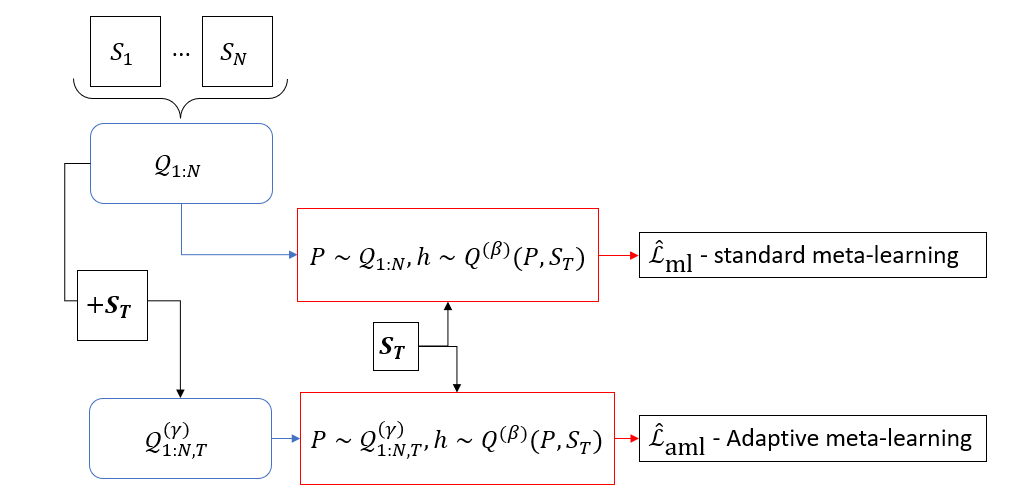
\includegraphics[width=\textwidth]{data_dependant_adaptation}
		\caption{Flowchart of meta-adaptation. A hyper-prior $\mathcal{Q}_{1:N}$ is learned from the training data. Standard meta-learning bounds use the test data to adapt the sampled prior before sampling a specific hypothesis. Our approach using data-dependent bounds also applies $S_T$ to the hyper-prior, resulting in a data-dependent hyper-posterior $\mathcal{Q}_{1:N, T}$. }
	\label{fig:data_dependant_bound}
	\end{subfigure}
	\hfill
	\caption{Standard meta-learning and meta-adaptation.}	 
\end{figure}

As we have seen, the meta-learning framework provides us with an informative hyper-posterior from which a good prior (i.e.\! one with low expected error) can be sampled. Given a specific downstream task $\mathcal{D}_T\sim \tau$ and a sample $S_T\sim \mathcal{D}^m$, we would like to provide a bound on the performance of any hyper-posterior that uses $S_T$, and the given hyper-prior $\mathcal{Q}_{1:N}$ that we previously meta-learned. In order to do so, we make use of PAC-Bayes bounds for data-dependent priors as the i.i.d.\ assumption common to PAC-Bayes bounds may not apply. As such, we re-state a known inequality from \citet{Rivasplata2020} and adapt it to the meta-learning setting

\begin{theorem} (PAC-Bayes for stochastic kernels - adapted from Theorem 2 in \citet{Rivasplata2020}) \label{thm:rivasplata-pb}
	Let $P\in \mathcal{K}(\mathcal{Z}^m, \mathcal{H})$ be a stochastic kernel (namely, this means $P$ may depend on the sampled data $S$), let $A: \mathcal{Z}^m\times \mathcal{H}\rightarrow \mathbb{R}^k$ be a measurable function for some positive integer $k$ and $F:\mathbb{R}^k\rightarrow \mathbb{R}$ be a convex function.
	Define $f\triangleq F\circ A$, and
	$$
	\xi(P_S, \mathcal{D}, f)=\int_{\mathcal{Z}^m}\int_{\mathcal{H}}e^{f(S, h)}P_S(dh)\mathcal{D}(dS),
	$$
	such that the data-dependent $P_S$ is the distribution over $\mathcal{H}$ corresponding to the sampled $S$. Assuming $\xi(P_S, \mathcal{D}, f)$ is finite (see below), then for any posterior $Q\in \mathcal{K}(\mathcal{Z}^m, \mathcal{H})$, with probability at least $1-\delta$ over the choice of $S\sim \mathcal{D}$
	\begin{equation} \label{eq:ribasplata-pb}
	\Expect{h\sim Q_S}{f(S, h)} \leq D_{KL}(Q_S||P_S)+\log\left (\xi(P_S, \mathcal{D}, f)/\delta\right ) .
	\end{equation}
\end{theorem}

An important but subtle distinguishing factor between this bound and classical PAC-Bayes bounds is that this bound applies to each individual posterior $Q_S$, but \emph{does not apply uniformly} to all posteriors. This seemingly minor difference means that the bound of \eqref{eq:ribasplata-pb} is not applicable for optimization over posteriors. Taking this limitation into account, this Theorem still provides an applicable upper bound on the expected loss for a given trained posterior. 

The term $\xi(P_S, \mathcal{D}, f)$ is known as the \emph{moment-generating function}, and, when it exists, it is an alternative specification of the probability distribution for $f$.
This moment-generating function intuitively quantifies the concentration of the function $f$ in the stochastic kernel $P\in{\cal K}({\cal Z}^m,{\cal H})$, and will be low if $f$ is well-concentrated.
The term $\log\xi(P_S, \mathcal{D}, f)$ is commonly referred to as the \emph{log-moment} and we will also do so throughout the rest of this paper for convenience. 
One simple setting where this term can be upper bounded is when the prior $P_S$ is data-free and $f(\cdot)\in[a,b]$. By switching the order of expectations (Fubini's theorem) and using Hoeffding's lemma, an upper bound for $f(S,h)=\lambda(\mathcal{L}(h,\mathcal{D})-\hat{\mathcal{L}}(h, S))$ for any $\lambda\in \mathbb{R}$ would be

\begin{align} 
    \mathbb{E}_{h\sim Q_S}&\left [\lambda(\mathcal{L}(h,\mathcal{D})-\hat{\mathcal{L}}(h, S))\right ]
     \leq D_{KL}(Q_S||P_S) \nonumber
    +\log\left (\frac{1}{\delta}\right ) + \frac{\lambda^2(b-a)^2}{8} .
\end{align}

Notably, this bound is similar to that of \citet{Catoni2004}. Other choices of $f$ result in other traditional PAC-Bayes bounds such as that of \citet{Mcallester} via similar methods (see \citet{Rivasplata2020} for further detail). 
One particularly appealing application of this general bound is for data-dependent priors with bounded log-moment terms, for example by conforming to certain algorithmic stability properties 
As an example for this notion, \citet{Rivasplata2020} show that for any prior satisfying the differential privacy property $DP(\epsilon)$, the log-moment can be upper bounded by the log-moment of a data-free prior plus a term that depends on the privacy parameter $\epsilon$. 

These data-dependent bounds can be applied to the meta-learning setting, giving us the following general result. 
%
\begin{theorem} \label{thm:main-result}
	Let $\mathcal{Q}_{1:N}\in \mathcal{M}(\mathcal{M}(\mathcal{H}))$ be a meta-learned hyper-posterior (e.g. the result of meta-training on $\{S_1,...,S_N\}$), and let $\mathcal{D}_T\sim \tau$ be a \emph{given} test task. Let $Q: \mathcal{Z}^m\times\mathcal{M}(\mathcal{H})\rightarrow \mathcal{M}(\mathcal{H})$ be a given base learner. Let $\ell: \mathcal{H}\times \mathcal{Z}\rightarrow [0, 1]$ be a bounded loss function.
	For any $\delta_T \in (0,1)$, for any hyper-posterior $\mathcal{Q}\in \mathcal{M}(\mathcal{M}(\mathcal{H}))$, and for all $\lambda>0$, with probability at least $1-\delta_T$ over the draw of $S_T\sim \mathcal{D}_T$:
	%
	\begin{align} \label{eq:main-result-generic}
	\begin{split}
	\mathcal{L}(\mathcal{Q}, \mathcal{D}_T) \leq \hat{\mathcal{L}}(\mathcal{Q}, S_T) + \frac{1}{\lambda}D_{KL}(\mathcal{Q}||\mathcal{Q}_{1:N})
	+\frac{1}{\lambda}\log\left ( \tilde{\xi}(\lambda,\mathcal{Q}_{1:N},\mathcal{D}_T)/\delta_T\right ) ,
	\end{split}
	\end{align}
%
	\begin{align*} 
	\begin{split}
	&\tilde{\xi}(\lambda,\mathcal{Q}_{1:N},\mathcal{D}_T)\triangleq 
	 \Expect{S\sim \mathcal{D}_T, P\sim \mathcal{Q}_{1:N}, h\sim Q(P,S)}{e^{\lambda\left (\mathcal{L}(h, \mathcal{D}_T)-\hat{\mathcal{L}}(h, S)\right )}} .
	\end{split}
	\end{align*}

\end{theorem}

The full proof of Theorem \ref{thm:main-result} is in Appendix \ref{append:proof-main-result}, and follows from Theorem \ref{thm:rivasplata-pb} using a two-level prior hypothesis $(\mathcal{Q}_{1:N}, Q)$. Concretely, we first sample $P\sim \mathcal{Q}_{1:N}$ and then sample $h\sim Q(P, S_T)$ to arrive at a hypothesis ,namely $Q$ is data-dependent. This two-level prior is compared to a two-level posterior $(\mathcal{Q}, Q)$, for any $\mathcal{Q}$. The proof itself applies even if the loss function $l$ is not bounded, but this assumption is very useful for providing bounds on the log-moment term.

This bound differs significantly from more traditional bounds that utilize a data-free two-level prior $(\mathcal{Q}_{1:N}, P)$. Such bounds apply uniformly over hyper-posteriors and are therefore suitable for optimization, but refer to the average loss on training tasks and contain additional complexity terms compared to \eqref{eq:main-result-generic} that result from using a data-free prior. An example of such a bound using Hoeffding's inequality is 
%
\begin{align} \label{eq:main-result-generic-datafree}
\begin{split}
\mathcal{L}(\mathcal{Q}, \mathcal{D}_T) &\leq \hat{\mathcal{L}}(\mathcal{Q}, S_T) 
+ \frac{1}{\lambda}D_{KL}(\mathcal{Q}||\mathcal{Q}_{1:N}) 
+ \frac{1}{\lambda}\Expect{P\sim \mathcal{Q}}{D_{KL}(Q(P,S_T)||P)}
+\frac{1}{\lambda}\log\frac{1}{\delta_T}+\frac{\lambda}{8m} .
\end{split}
\end{align}

%This more traditional bound contains an additional complexity term between prior and posterior $D_{KL}(Q(P,S_T)||P)$, but since $P$ is independent from $S_T$, the moment-generating function can be easily bounded. This can be seen as a trade-off between the part of the bound that can be optimized by the choice of posterior $\mathcal{Q}$ and the term in the bound that results from the log-moment.

One immediate result of \eqref{eq:main-result-generic} is a bound on the expected error of the hyper-prior for the downstream task, achieved by picking $\mathcal{Q}=\mathcal{Q}_{1:N}$, and appears in Corollary \ref{thm:corollary-base}.

It is important to note that the log-moment term $\log\tilde{\xi}(\lambda,\mathcal{Q}_{1:N},\mathcal{D}_T)$ is a key term in both cases. It will be low if the empirical losses are well concentrated around the expected loss for our data-dependent prior. One possible method of achieving this is by choosing a base learner $Q$ with algorithmic stability properties such as the empirical Gibbs posterior, as we will see in the next subsection.

%Unlike standard meta-learning bounds discussed in Section \ref{sec:meta}, the right-hand side for this bound contains the empirical loss on data from the test task, making straightforward comparison between these bounds effectively impossible. The bound in Corollary \ref{thm:corollary-base} can be thought of as a confidence bound for the expected loss whereas the bound in Theorem \ref{thm:meta-highprob} provides a PAC-Bayes bound based on the data-free hyper-prior and the average training loss.

\subsection{Meta-adaptation with Gibbs posteriors} \label{sec:adapt-gibbs}
%meta-train, meta-test with Gibbs

One class of hyper-posteriors that is especially appealing for analysis given Theorem \ref{thm:main-result} is the class of Gibbs posteriors.

\begin{defn} \label{defn:Gibbs}
	The Gibbs distribution with parameter $\beta>0$ is defined as 
	\begin{equation}\label{eq:GibbsDef}
	    Q^\beta(P,S)(h)=\frac{P(h)e^{-\beta \hat{\mathcal{L}}(h,S)}}{\Expect{h\sim P}{e^{-\beta\hat{\mathcal{L}}(h,S)}}}~.
	\end{equation}
\end{defn}

It is well-known \citep{Catoni2004} that given a specific value for $\lambda$, using Donsker and Varadhan’s variational formula \citep{Donsker1975} provides the hyper-posterior that minimizes the right-hand side of \eqref{eq:main-result-generic}, given by
%
\begin{equation*}
    \mathcal{Q}^{\lambda}_{1:N,T}=\frac{\mathcal{Q}_{1:N}e^{-\lambda\hat{\mathcal{L}}(Q,S_T)}}{\Expect{P\sim \mathcal{Q}_{1:N}}{e^{-\lambda\hat{\mathcal{L}}(Q,S_T)}}}~.
\end{equation*}
The meaning of this result is that given that we know the relative importance of the empirical loss and the KL-divergence, the optimal hyper-posterior that minimizes \eqref{eq:main-result-generic} is the Gibbs hyper-posterior $\mathcal{Q}^{\lambda}_{1:N,T}$.

This property encourages further exploration of the Gibbs hyper-posterior for meta-adaptation. Using \eqref{eq:GibbsDef}, we define 
\begin{equation} \label{eq:aml-post-defn}
\mathcal{Q}^{\gamma}_{1:N,T}\triangleq \frac{\mathcal{Q}_{1:N}e^{-\gamma\hat{\mathcal{L}}(Q^\beta(P,S_T),S_T)}}{Z_\gamma(S_T, \mathcal{Q}_{1:N})} \qquad ; \qquad Z_\gamma(S_T, \mathcal{Q}_{1:N})\triangleq \Expect{P\sim \mathcal{Q}_{1:N}}{e^{-\gamma\hat{\mathcal{L}}(Q^\beta(P,S_T),S_T)}}
\end{equation} 
as the Gibbs posterior for the meta-learned problem. 
$\mathcal{Q}^{\gamma}_{1:N,T}$ is a specific case of $\mathcal{Q}^{\lambda}_{1:N,T}$ where the base learner is a Gibbs posterior.
We have 
\begin{align*} 
\begin{split}
D_{KL}(\mathcal{Q}^{\gamma}_{1:N,T}||\mathcal{Q}_{1:N})&=
-\gamma\hat{\mathcal{L}}(\mathcal{Q}_{1:N,T}, S_T)
-\log Z_\gamma(S_T, \mathcal{Q}_{1:N}) .
\end{split}
\end{align*}

So plugging these values in \eqref{eq:main-result-generic} gives us
\begin{align*} 
\begin{split}
\mathcal{L}(\mathcal{Q}^{\gamma}_{1:N,T}, \mathcal{D}_T) & \leq \hat{\mathcal{L}}(\mathcal{Q}^{\gamma}_{1:N,T}, S_T) -\frac{\gamma}{\lambda}\hat{\mathcal{L}}(\mathcal{Q}^{\gamma}_{1:N,T}, S_T) - \frac{1}{\lambda}\log Z_\gamma(S_T, \mathcal{Q}_{1:N}) +\frac{1}{\lambda}\log\left (\tilde{\xi}(\lambda,\mathcal{Q}_{1:N},\mathcal{D}_T)/\delta_T\right ) .
\end{split}
\end{align*}

In order to clarify this expression, we will use more intuitive definitions for our empirical losses.
\begin{defn}
	The adapted meta-loss (AML) is  
	\begin{align*} 
	\hat{\mathcal{L}}_{\mathrm{aml}} (\mathcal{Q}^{\gamma}_{1:N,T}, S_T)
	&=\mathbb{E}_{P\sim \mathcal{Q}^{\gamma}_{1:N,T}}\mathbb{E}_{h\sim Q^{\beta}(P,S_T)}\left [\hat{\mathcal{L}}(h, S_T)\right ]
	\end{align*} 
	meaning that $S_T$ is used to adapt both the hyper-prior ($\mathcal{Q}_{1:N}$) and the sampled prior that depends on $S_T$. $\hat{\mathcal{L}}_{\mathrm{aml}}$ is a function of both $\gamma$ and $\beta$. The standard meta-loss 
	$$
	\hat{\mathcal{L}}_{\mathrm{ml}}(\mathcal{Q}_{1:N}, S_T)=\mathbb{E}_{P\sim \mathcal{Q}_{1:N}}\mathbb{E}_{h\sim Q^{\beta}(P,S_T)}\left [\hat{\mathcal{L}}(h, S_T)\right ]~, 
	$$ 
	is the empirical loss of the base learner using the basic meta-learning hyper-prior $\mathcal{Q}_{1:N}$. 
	$\hat{\mathcal{L}}_{\mathrm{ml}}$ depends on $\beta$, but not on $\gamma$.
\end{defn}

Using these definitions, we have:

\begin{align*} 
\begin{split}
\mathcal{L}(\mathcal{Q}_{1:N,T}, \mathcal{D}_T) &\leq  (1-\frac{\gamma}{\lambda})\hat{\mathcal{L}}_{\mathrm{aml}} (\mathcal{Q}^{\gamma}_{1:N,T}, S_T) - \frac{1}{\lambda}\log \mathbb{E}_{P\sim \mathcal{Q}_{1:N}}\left [e^{-\gamma\hat{\mathcal{L}}(Q^\beta(P,S_T),S_T)}\right ]
+\frac{1}{\lambda}\log\left (\tilde{\xi}(\lambda,\mathcal{Q}_{1:N},\mathcal{D}_T)/\delta_T\right ) .
\end{split}
\end{align*}

By simplifying the second term using Jensen's inequality, we arrive at the following theorem.

\begin{corollary} \label{thm:main-result-gibbs}
	Let $\mathcal{Q}_{1:N}$ be a hyper-posterior (e.g. the result of meta-training on $\{S_1,...,S_N\}$), and let $\mathcal{D}_T\sim \tau$ be a given test task. Define  $\mathcal{Q}^\gamma_{1:N,T}$ as in \eqref{eq:aml-post-defn}. 
	For all $\lambda>0, \gamma>0$, 
	with probability at least $1-\delta_T$ over the draw of $S_T\sim \mathcal{D}_T$:
	
	\begin{align} \label{eq:pb-adapt-multi}
	\begin{split}
	\mathcal{L}(\mathcal{Q}_{1:N,T}, \mathcal{D}_T) &\leq 
	(1-\frac{\gamma}{\lambda})\hat{\mathcal{L}}_{\mathrm{aml}} (\mathcal{Q}^{\gamma}_{1:N,T}, S_T) + \frac{\gamma}{\lambda}\hat{\mathcal{L}}_{\mathrm{ml}}(\mathcal{Q}_{1:N}, S_T) 
	+\frac{1}{\lambda}\log\left (\tilde{\xi}(\lambda,\mathcal{Q}_{1:N},\mathcal{D}_T)/\delta_T\right ) .
	\end{split}
	\end{align}
\end{corollary}

In order to better understand the impact of the log-moment term, we remark that \citet{Rivasplata2020} have shown that for $\lambda=\sqrt{m}$ and given that the base learner is the empirical Gibbs posterior $Q^\beta$ and the loss is bounded,

$$\log\tilde{\xi}(\sqrt{m},\mathcal{Q}_{1:N},\mathcal{D}_T) \leq 2+\log(1+\sqrt{e})+\frac{2\beta}{\sqrt{m}} .$$

As a consequence of this, choosing $\beta=\sqrt{m}$ would result 
in the log-moment to be bounded by a constant $C$. Consequentially, the bound takes the form
    \begin{align*}
    \begin{split}
    \mathcal{L}(\mathcal{Q}_{1:N,T}, \mathcal{D}_T) &\leq \hat{\mathcal{L}}_{\mathrm{aml}} (\mathcal{Q}^{\gamma}_{1:N,T}, S_T) +
    \frac{\gamma}{\sqrt{m}}\left (\hat{\mathcal{L}}_{\mathrm{ml}}(\mathcal{Q}_{1:N}, S_T)-\hat{\mathcal{L}}_{\mathrm{aml}} (\mathcal{Q}^{\gamma}_{1:N,T}, S_T)\right ) 
+\frac{1}{\sqrt{m}}\log\frac{1}{\delta_T}+\frac{C}{\sqrt{m}} .
    \end{split}
    \end{align*}
%Evidently from this bound, the generalization gap (the difference $\mathcal{L}(\mathcal{Q}_{1:N,T}, \mathcal{D}_T)-\hat{\mathcal{L}}_{\mathrm{aml}}$) is of rate $O\left (\frac{1}{\sqrt{m}}\right )$.


Corollary \ref{thm:main-result-gibbs} provides an upper bound on the expected error for a given test task that depends on the empirical errors of the hyper-prior $\hat{\mathcal{L}}_{\mathrm{ml}}$ and the hyper-posterior $\hat{\mathcal{L}}_{\mathrm{aml}}$. 
Since the bound applies uniformly for all $\gamma>0,\beta>0,\lambda>0$, this bound can be further improved by choosing optimal values for $\gamma, \beta, \lambda$ through optimization algorithms such as gradient descent w.r.t.\! these parameters.

\subsection{Tighter bounds for the low error setting}
% seeger

Theorem \ref{thm:main-result} is the result of applying the generic data-dependent bound (Theorem \ref{thm:rivasplata-pb}) with the measurement function $f=\lambda(\mathcal{L}(\mathcal{Q},\mathcal{D}_T)-\hat{\mathcal{L}}(\mathcal{Q}, S_T))$. For cases where $\hat{\mathcal{L}}(\mathcal{Q}, S_T)$ is low, it may be better to use a bound based on the binary KL-divergence $f=\lambda \mathrm{kl}(\hat{\mathcal{L}}(\mathcal{Q}, S_T)||\mathcal{L}(\mathcal{Q},\mathcal{D}_T))$, 
$$
\mathrm{kl}(q||p)=q \log\frac{q}{p}+(1-q)\log\frac{1-q}{1-p},\;\;\; q,p\in[0, 1]
$$
Doing so gives the upper bound
    \begin{align} \label{eq:generic-kl-bound}
\begin{split}
\mathrm{kl}(\hat{\mathcal{L}}(\mathcal{Q}, S_T)||\mathcal{L}(\mathcal{Q},\mathcal{D}_T)) &\leq \frac{1}{\lambda} D_{KL}(\mathcal{Q}||\mathcal{Q}_{1:N})
+\frac{1}{\lambda}\log\left (\bar{\xi}_{\mathrm{kl}}/\delta_T\right ) 
\end{split}
\end{align}

where $\bar{\xi}_{\mathrm{kl}}\triangleq \bar{\xi}(\mathcal{Q}_{1:N}, \mathcal{D}_T,\lambda, \mathrm{kl}) .$

If the base learner $Q$ is the Gibbs posterior (\eqref{eq:GibbsDef}), the moment term of  \eqref{eq:generic-kl-bound} can be meaningfully bounded. To do so, we make use of the notion of differential privacy at scale $\epsilon$, $DP(\epsilon)$ (see Definition \ref{def:diff_privacy} in the appendix).

It has been proven \citep{McSherry2007, Rivasplata2020} that the Gibbs posterior $Q(P, S)(h)\propto P(h)e^{-\beta\hat{\mathcal{L}}(h, S)}$ is $DP\left (\frac{2\beta}{m}\right )$.
This result can be extended to the meta-learning setting as follows. 
%
\begin{proposition} \label{thm:pair-is-dp}
	Let $\mathcal{P}\in \mathcal{M}(\mathcal{M}(\mathcal{H}))$ be a hyper-prior.
	Let $\ell:\mathcal{H}\times \mathcal{Z}\rightarrow [0,1]$ be a bounded loss function. If the base learner $Q\in \mathcal{M}(\mathcal{H})$ is the Gibbs posterior $Q(P, S)(h)\propto P(h)e^{-\beta\hat{\mathcal{L}}(h, S)}$, 
	then the pair hypothesis $(\mathcal{P}, Q)$ that samples $P\sim\mathcal{P}$ and $h\sim Q(P, S)$ satisfies $DP\left (\frac{2\beta}{m}\right )$.
\end{proposition}

The proof of Proposition \ref{thm:pair-is-dp} is in Appendix \ref{append:proof-dp}. This  allows us to extend an existing result for PAC-Bayes with private data-dependent priors.
By making use of Theorem 4.2 in \citet{Dziugaite2018} as well as  \eqref{eq:generic-kl-bound} with $\lambda=m$, we get the following Theorem.

\begin{theorem} \label{thm:kl-main-result}
	Let $\ell:\mathcal{H}\times \mathcal{Z}\rightarrow [0,1]$ be a bounded loss function.
	Let $\mathcal{Q}_{1:N}$ be a hyper-posterior (e.g. the result of meta-training on $\{S_1,...,S_N\}$), and let $\mathcal{D}_T\sim \tau$ be a given test task. 
	If the base learner $Q\in \mathcal{M}(\mathcal{H})$ is the Gibbs posterior $Q(P, S)(h)\propto P(h)e^{-\beta\hat{\mathcal{L}}(h, S)}$, 
	for any $\delta\in(0,1)$, uniformly for all hyper-posteriors $\mathcal{Q}\in \mathcal{M}(\mathcal{M}(\mathcal{H}))$, with probability at least $1-\delta$ over the draw of $S_T\sim \mathcal{D}_T$,
%
	\begin{align*} 
	\begin{split}
	\mathrm{kl}(\hat{\mathcal{L}}(\mathcal{Q},S_T)||\mathcal{L}(&\mathcal{Q},\mathcal{D}_T))\leq \frac{2\beta^2}{m^2}+\frac{\beta}{m}\sqrt{\frac{2\log (4/\delta_T)}{m}} 
	+\frac{1}{m}\left (D_{KL}(\mathcal{Q}||\mathcal{Q}_{1:N})+\log\frac{4\sqrt{m}}{\delta_T} \right ) .
	\end{split}
	\end{align*}
\end{theorem}

%=================================================================================
\subsection{Empirical evaluation}

Since Theorem \ref{thm:main-result} does not apply uniformly over hyper-posteriors, we cannot derive a practical optimization algorithm just by minimizing the right-hand side of  \eqref{eq:main-result-generic}. 
One way to resolve this issue is to add a base-learner complexity term $\frac{1}{\lambda}\Expect{P\sim \mathcal{Q}}{D_{KL}(Q||P)}$ to  \eqref{eq:main-result-generic}, thus arriving at \eqref{eq:main-result-generic-datafree} that applies to data-free priors, and derive optimizable meta-adaptation bounds based on it.
Another method to address this issue is to use bounds such as Theorem 4.2 of \citet{Dziugaite2018} that apply uniformly for all posteriors, but only for specific classes of data-dependent priors, in this case differentially-private ones.
Another potential solution to this issue is to split the provided data $S_T$ into disjoint adaptation and evaluation sets, $S_{\mathrm{adapt}}$ and $S_{\mathrm{eval}}$, during the meta-adaptation phase, and learn the posterior $Q$ based on the adaptation set $S_{\mathrm{adapt}}$ alone. Since this is already common practice in meta-learning algorithms (e.g.\ sampling different data points for the meta-update step \citet{Finn2017}), we chose to do so for our empirical evaluation. %Future work will consider and compare these solutions.

We use stochastic neural networks \citep{Graves2011, Blundell2015} similarly to the MLAP \citep{Amit2018} algorithm, and consider meta-adaptation with three different hyper-priors. \emph{(i)} The meta-learned hyper-prior $\mathcal{Q}_{1:N}$. \emph{(ii)} A zero-centered stochastic neural network. \emph{(iii)}  An adaptive hyper-prior based on the last optimization loop, as described in algorithm \ref{alg1}, and in more detail in Appendix \ref{append:hyper-params}. 

Algorithm \ref{alg1} describes the meta-adaptation algorithm for stochastic neural networks using $\theta$ to mark the meta-learner parameters and $\phi$ to mark the base learner parameters. The standard meta-testing algorithm that is used to adapt a sampled prior to a given task is described in Appendix \ref{append:hyper-params}. We use a slight abuse of notation $\phi\sim \theta$ to denote sampling according to the parametric distribution defined by the stochastic neural network.

\begin{algorithm}[H]
	\caption{Meta-adaptation}
	\label{alg1}
	\small
	\begin{algorithmic}
		\Function{Meta-adapt}{$\theta_{1:N}$, $S_T\sim \mathcal{D}_T$}
		\State Choose algorithmic parameters $\eta_\alpha, K, \lambda, N_{MC}$
		\State Initialize $\hat{\theta}_{1:N, T}\leftarrow \theta_{1:N}$
		\While {Not converged} \Comment Or limit number of epochs
		\State Sample $\hat{\phi}_1,\ldots,\hat{\phi}_K\sim \hat{\theta}_{1:N, T}$
		\For {each meta-batch $k$ from $1$ to $K$} 
		\State Set $S_k\leftarrow S_T$
		\State Split $S_k$ to $S_{k,\mathrm{adapt}},S_{k,\mathrm{eval}}$
		\For {each Monte-Carlo estimation $j$ from $1$ to $N_{MC}$} 
		\State Sample $h_j\sim \hat{\phi}_k$
		\State Calculate $L_{kj}(h_j, S_{k,\mathrm{eval}})=\hat{\mathcal{L}}(h_j,S_{k,\mathrm{eval}})$
		\EndFor 
		\State $J_k(L_{kj}, \hat{\theta}_{1:N, T}, \lambda,\hat{\phi}_k )=\frac{1}{N_{MC}}\sum_{j=1}^{N_{MC}}L_{kj}+\frac{1}{\lambda} D_{KL}(\hat{\phi}_k||\hat{\theta}_{1:N,T})$ \Comment $S_{k,\mathrm{adapt}}$ can be used to optimize $\lambda$ w.r.t. $J_k$
		\EndFor
		\State $J(\hat{\theta}_{1:N,T}, \hat{\phi}_1,\ldots,\hat{\phi}_K, \lambda, J_1,\ldots,J_K)=\frac{1}{K}\sum_{k=1}^{K}J_k + \frac{1}{\lambda} D_{KL}(\hat{\theta}_{1:N, T}||\hat{\theta}_{1:N})$
		\State  Run SGD step w.r.t $\hat{\theta}_{1:N, T},\hat{\phi}_1,\ldots,\hat{\phi}_K$ on $J$
		\EndWhile
		\State \Return $\hat{\theta}_{1:N, T}$
		\EndFunction
	\end{algorithmic}
\end{algorithm}

Since we tested our approach on neural networks, the hypothesis space is defined as $\{h(w)|w\in \mathbb{R}^d\}$, where the weights $w$ serve as the parameters of each hypothesis.
For image classification tasks, $x$ represents an image, and $y$ a class label. 
We use the cross-entropy loss during adaptation, despite the fact that it is not bounded. We note that a clipped variation of this loss does exist, and conforms to theoretical guarantees \citep{Dziugaite2018}, and that in practice the cross-entropy loss tends to be low. 

We first conduct experiments on a task environment based on the MNIST dataset \citep{LeCun1998}, where each task was created by performing a random permutation on some of the image pixels. The number of pixels to be shuffled and the total number of classes (referred to as ``ways'') was chosen in advance. In order to obtain a reasonable hyper-prior $\mathcal{Q}_{1:N}$ on downstream tasks, it makes sense to run standard meta-training methods on the training data.
We used the MLAP \citep{Amit2018} algorithm to do so. We ran MLAP-M for 100 meta-training iterations on randomly sampled training tasks, with 100 examples from each class. The resulting network means and variances were then used as the final meta-training hyper-prior $\mathcal{Q}_{1:N}$. We used the same convolutional neural network (CNN) architecture used by \citet{Vinyals2016} for the Omniglot dataset.

We perform tests on two sets of problems, tasks with $100$ shuffled pixels, and tasks with permuted labels instead of pixels.
For standard meta-testing, we sample a prior $P\sim \mathcal{Q}_{1:N}$ and perform $1000$ adaptation steps given the labeled adaptation dataset $S_T$ in order to achieve convergence. For our meta-adaptation method, we initialize the hyper-posterior as the meta-training hyper-prior $\mathcal{Q}_{1:N}$ and
 perform several steps of meta-adaptation as detailed in Algorithm \ref{alg1}. Following that, we sample a prior $P\sim \mathcal{Q}_{1:N,T}$ and perform  $50$ SGD steps of standard meta-testing. Since the meta-adaptation process itself includes computational costs, we use far fewer update steps for the sampled prior in order to have a fairer comparison.
See appendix \ref{append:hyper-params} for a full list of hyper-parameters and implementation details.

Figure \ref{fig:results-pixels} shows the test accuracy averaged over $10$ meta-testing seeds for both tasks.
Numerical values for both tasks as well as standard error are reported in Table \ref{table:gamma}. Significant improvements for the Wilcoxon test $(p<0.05)$ are marked with *.  Empirical results for the MNIST tasks show that meta-adaptation is preferable to standard meta-testing for relatively small adaptation set sizes by a notable margin.


\begin{figure}[h!]
	\centering
	\begin{subfigure}[b]{0.49\textwidth}
		\centering
		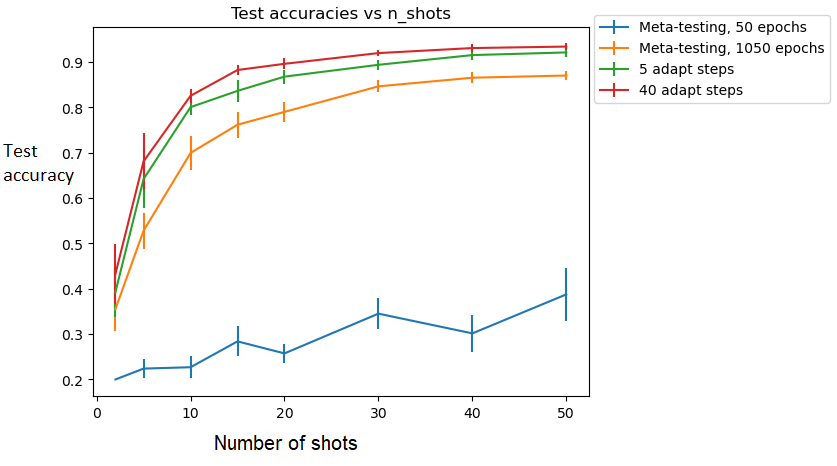
\includegraphics[width=\textwidth]{test_accuracies_pixels_const}
		\caption{Meta Adaptation - shuffled pixels}
	\end{subfigure}
	\hfill
	\begin{subfigure}[b]{0.49\textwidth}
		\centering
		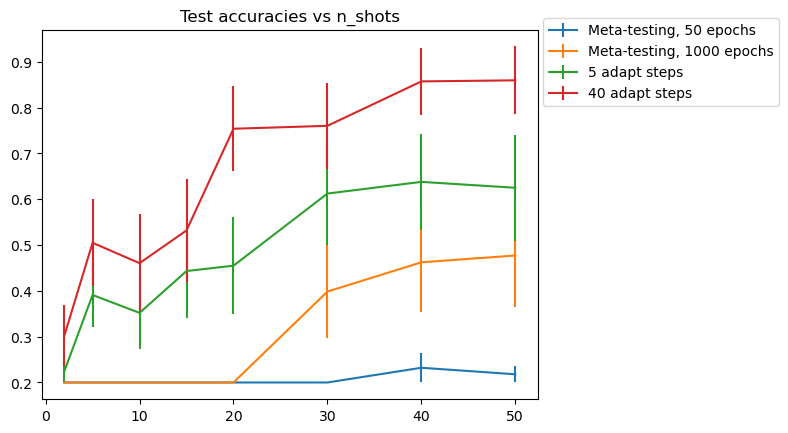
\includegraphics[width=\textwidth]{test_accuracies_labels_const}
		\caption{Meta Adaptation - permuted labels}	 	
	\end{subfigure}
	\hfill
	\caption{Average test accuracies on both MNIST tasks, for meta-adaptation with varying gradient updates. Error bars represent standard errors from the mean over $10$ runs.}	 
	\label{fig:results-pixels}
\end{figure}


\begin{figure}[h!]
	\centering
	\begin{subfigure}[b]{0.4\textwidth}
		\centering
		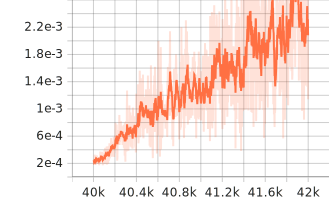
\includegraphics[width=\textwidth]{kl_adaptive}
		\caption{$D_{\mathrm{KL}}(\mathcal{Q}_{1:N,T}||\mathcal{Q}_{1:N})$ over training epochs, smoothed.}
	\end{subfigure}
	\hfill
	\begin{subfigure}[b]{0.4\textwidth}
		\centering
		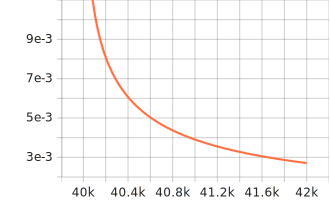
\includegraphics[width=\textwidth]{kl_normal}
		\caption{$D_{\mathrm{KL}}(\mathcal{Q}_{1:N,T}||\mathcal{N}(0,I_d))$ over training epochs.}	 	
	\end{subfigure}
	\hfill
	\caption{KL-divergences during the meta-adaptation process for the mini-Imagenet dataset.}	 
	\label{fig:results-kls}
\end{figure}

\begin{table*}[t]	
	\caption{Test accuracies for the meta-MNIST dataset.}
	\label{table:gamma}
	\begin{center}
	\begin{tabular}{llll}
		Method   & N\_shots  & Shuffled-pixels & Permuted-labels  
  \\ \hline \\
		
		MLAP-M  & $5$   & $0.53\pm 0.04 $   & $0.2\pm 0 $   \\
		Meta-adaptation & $5$   & $0.68^*\pm 0.06 $ & $0.51^*\pm 0.1 $ \\
		\midrule
		MLAP-M  & $10$   & $0.7\pm 0.04 $   & $0.2\pm 0.0 $   \\
		Meta-adaptation & $10$   & $0.83^*\pm 0.02 $ & $0.461\pm 0.106 $ \\
		\midrule
		MLAP-M  & $20$   & $0.79\pm 0.02 $   & $0.2\pm 0.0 $   \\
		Meta-adaptation & $20$   & $0.9^*\pm 0.01 $ & $0.75^*\pm 0.09 $ \\
		\midrule
		MLAP-M  & $50$   & $0.87\pm 0.01 $   & $0.48\pm 0.11 $   \\
		Meta-adaptation & $50$   & $0.93^*\pm 0.01 $ & $0.86^*\pm 0.07 $ \\
		\bottomrule
	\end{tabular}
        \end{center}
	
\end{table*}

\begin{table*}[t]	
	\caption{Test accuracies for the mini-Imagenet dataset. }
	\label{table:inet}
	\centering
	\begin{tabular}{lll}
		
		Method   & N\_shots  & Test accuracy \% \\ \hline \\
		MAML \citep{Finn2017}& $5$   & $63.15 \pm 0.91 $      \\
		VAMPIRE \citep{nguyen2020} & $5$   & $64.31 \pm 0.74 $ \\
		Bayesian-VI & $5$   & $52.8\pm 3.6 $    \\
		Meta-adaptation & $5$   & $60\pm 2.6 $ \\
		\midrule
		Bayesian-VI & $20$   & $61.7\pm 2.2$     \\
		Meta-adaptation & $20$   & $64.9^* \pm 1.7 $  \\
		\midrule
	\end{tabular}
	
\end{table*}

Table \ref{table:inet} compares test accuracies for the well-known mini-Imagenet \citep{Vinyals2016} dataset. Results for MAML \citep{Finn2017} and VAMPIRE \citep{nguyen2020} are from their respective papers, results for Bayesian variational inference (VI) and meta-adaptation are averaged over $5$ seeds with standard error reported. Since fewer seeds were used, results have a higher standard error. While our empirical results are not better than existing SoTA meta-learning algorithms, they are comparable and show an improvement beyond standard meta-testing for relatively low adaptation set size $|S_T|$. Better hyper-parameter tuning may be needed in order to achieve improved results. As $|S_T|$ increases, the training loss becomes a better estimate of the expected loss for the task, leading to a better base learner as well as more reliable improvements from meta-adaptation. 

Figure \ref{fig:results-kls} shows the typical progression of KL-divergence during the meta-adaptation fitting process. We see that $D_{\mathrm{KL}}(\mathcal{Q}_{1:N,T}||\mathcal{N}(0,I_d))$ decreases (alongside the training loss on the adaptation data), resulting in lower overall variance in network weights as well as a shift in the means. $D_{\mathrm{KL}}(\mathcal{Q}_{1:N,T}||\mathcal{Q}_{1:N})$ tends to increase slowly during meta-adaptation, resulting in a hyper-posterior that diverges from the original meta-learned hyper-prior as the training loss decreases. A different choice of hyper-parameters for $\lambda$ may cause this term to diverge more slowly, leaving us with a more similar hyper-posterior.

Results for the Omniglot \citep{Vinyals2016} dataset were ommitted since all approaches reached results above $99\%$ accuracy for the $5$-shot $5$-way setting. 

\section{Discussion and Future Work}

We have derived several PAC-Bayes generalization bounds for meta-testing based on data-dependent bounds, and have demonstrated the efficacy of using the adaptation data in order to create a more appropriate hyper-posterior for a new test task.
We have implemented a practical algorithm based on the derived bounds and have demonstrated its efficacy in few-shot image classification. To the best of our knowledge, our approach is the first meta-learning algorithm to consider adapting a learned hyper-prior in a principled approach.

While our experimental results are preliminary, they clearly demonstrate an improvement in terms of generalization error for the MNIST dataset, and results comparable to other well-known meta-learning algorithms (MAML, VAMPIRE) for the Omniglot and mini-Imagenet datasets with similar hypothesis classes. Future work should evaluate whether better parameter tuning can bridge the gap between meta-adaptation and SoTA results, as well as considering results for datasets with more pronounced distirbution shifts between training and testing.

There are two main open issues to be addressed in future work. 
The first issue is that our approach requires the use of stochastic models, which may lead to high-variance gradients and are therefore non-trivial to optimize. One potential method to address this issue is to make use of PAC-Bayes bounds with different complexity measures such as Wasserstein distance \citep{Ohnishi2021, Amit2022}.
The second issue is to consider our meta-adaptation algorithm in the context of continual learning \citep{Kirkpatrick2017}. Recent work by \citet{Haddouche2022} used data-dependent PAC-Bayes bounds in the context of online learning, and it would be of interest to extend these results to the continual setting and derive bounds that provide a clearer tradeoff between low generalization error and avoiding catastrophic forgetting

%\clearpage
%\bibliographystyle{aaai23}
\bibliographystyle{collas2023_conference}
\bibliography{library}

\clearpage
\appendix 
\section{Appendix}
\label{sec:appendix}

\subsection{Hyper-parameters and implementation details} \label{append:hyper-params}

\begin{algorithm}[H]
	\caption{Standard Meta-testing}
	\small
	\begin{algorithmic}
		\Function{Meta-test}{$\theta$, $S_T\sim \mathcal{D}_T$}
		\State Choose algorithmic parameters $\eta_\alpha, \#$ steps, $c$
		\State Sample $\phi\sim \mathcal{N}(\theta)$
		\While {test step $<$ $\#$ steps} \Comment Proxy to convergence
			\State $J(\phi, S_T,\theta)=\hat{\mathcal{L}}(\phi, S_T) + D_{KL}(\phi||\theta) + c\cdot D_{KL}(\phi||(0,\sigma^2 I))$ \Comment $D_{KL}(\phi||(0,\sigma^2 I))$ is a low-norm condition on $\phi$
			\State  Take gradient step of size $\eta_\alpha$ w.r.t.\! $\phi$ on $\nabla J$

		\EndWhile
		\State \Return $\phi$
		\EndFunction
	\end{algorithmic}
\end{algorithm}

In the adaptive hyper-posterior version of the meta-adaptation algorithm, we first initialize the hyper-posterior $\hat{\mathcal{Q}}_{1:N, T}$ to the meta-training hyper-prior $\mathcal{Q}_{1:N}$. In each adaptation step, we optimize \eqref{eq:main-result-generic-datafree} w.r.t.\! $\hat{\mathcal{Q}}_{1:N, T},\hat{Q}$ and perform gradient updates on the hyper-posterior. We then set the hyper-prior for the next adaptation step as the current hyper-posterior.
In the constant hyper-prior version of the meta-adaptation algorithm, the hyper-prior remains the same throughout the meta-adaptation process.

The network architecture used for classification on the permuted MNIST dataset is identical to that used for the Omniglot dataset by \citet{Vinyals2016}: $4$ layers of $2$D $3\times 3$ convolution layers followed by batch norm and max pooling each. These are followed by a linear classification layer with $5$ classes (commonly referred to as number of ways). The training loss used was standard cross-entropy loss. We used the Adam optimizer \citep{Kingma2015} for meta-training and meta-testing. 
Code to reproduce the experiments will be made available after publication.
%Code to reproduce the experiments is available at https://github.com/lioritan/meta-adapt-pb.\RM{Should be anonymous. Promise to provide after publication.}

\begin{table*}[ht]	
	
	\centering
 \caption{Hyper-parameter choices, MNIST}
	\label{table:hyper-params}
	\begin{tabular}{lll}
		
		Notation   & Description  & Value/s   \\ \hline \\
		\#Training epochs & Number of training epochs for hyper-prior   & $100$      \\
		\midrule
		Train Sample size & \# of training examples per class per epoch   & $100$      \\
		\midrule
		\#Test epochs & Number of base learner gradient updates   & $50,1000$      \\
		\midrule
		$\eta_{\alpha}$  & Learning rate for the meta-learner   & $0.01$      \\
		\midrule
		$\eta_{\beta}$  & Learning rate for the base learner   & $0.1$      \\
		\midrule
		\#Adaptation steps  & Number of training epochs for hyper-posterior   & $5,40$      \\
		\midrule
		MC-iterations & Number of Monte-Carlo samples to average & $3$\\
		\midrule
		Test permutations  & Number of pixels permuted on each test image   & $100$      \\
		\midrule
		\#ways & Number of classes in classification & $5$\\
		\midrule
		\#shots & Number of samples per class in $S_T$ & $2,5,10,15,20,30,40,50$\\
		\midrule
		seed & Random seed, chosen arbitrarily & $42,1337,7,13,999,752,56789,145790,11,306050$\\
		\bottomrule
	\end{tabular}
\end{table*}

\begin{table*}[ht]	
	
	\centering
 \caption{Hyper-parameter choices, mini-Imagenet}
	\label{table:hyper-params-inet}
	\begin{tabular}{lll}
		
		Notation   & Description  & Value/s   \\ \hline \\
		\#Training epochs & Number of training epochs for hyper-prior   & $20000$      \\
		\midrule
		Train Sample size & \# of training examples per class per epoch   & $20$      \\
		\midrule
		\#Test epochs & Number of base learner gradient updates   & $5$      \\
		\midrule
		$\eta_{\alpha}$  & Learning rate for the meta-learner   & $0.001$      \\
		\midrule
		$\eta_{\beta}$  & Learning rate for the base learner   & $0.01$      \\
		\midrule
		\#Adaptation steps  & Number of training epochs for hyper-posterior   & $1000, 2000$      \\
		\midrule
		MC-iterations & Number of Monte-Carlo samples to average & $10$\\
		\midrule
		\#ways & Number of classes in classification & $5$\\
		\midrule
		\#shots & Number of samples per class in $S_T$ & $5,20$\\
		\midrule
		seed & Random seed, chosen arbitrarily & $11,13,999,56789,306050$\\
		\bottomrule
	\end{tabular}
	
\end{table*}

\subsection{Proof of the generic meta-adaptation bound} \label{append:proof-main-result}

We restate Theorem \ref{thm:rivasplata-pb} for stochastic kernels. 

\begin{theorem} (PAC-Bayes for stochastic kernels - adapted from Theorem 2 in \citet{Rivasplata2020}) \label{thm:rivasplata-pb-appendix}
	Let $P\in \mathcal{K}(\mathcal{Z}^m, \mathcal{H})$ be a stochastic kernel (namely, the prior may depend on the sample data $S$), let $A: \mathcal{Z}^m\times \mathcal{H}\rightarrow \mathbb{R}^k$ be a measurable function for some positive integer $k$ and $F:\mathbb{R}^k\rightarrow \mathbb{R}$ be a convex function.
	Define $f\triangleq F\circ A$, and  
	$$
	\xi(P_S, \mathcal{D}, f)=\int_{\mathcal{Z}^m}\int_{\mathcal{H}}e^{f(S, h)}P_S(dh)\mathcal{D}(dS) , 
	$$
	such that $P_S$ is the distribution over $\mathcal{H}$ corresponding to the sampled $S$. Assuming $\xi(P_S, \mathcal{D}, f)$ is finite, then for any $\delta \in (0,1)$ and any posterior $Q\in \mathcal{K}(\mathcal{Z}^m, \mathcal{H})$, with probability at least $1-\delta$ over the choice of $S\sim \mathcal{D}$,
	\begin{equation} \label{eq:ribasplata-pb-appendix}
	\Expect{h\sim Q_S}{f(S, h)} \leq D_{KL}(Q_S||P_S)+\log\left (\xi(P_S, \mathcal{D}, f)/\delta\right ) .
	\end{equation}
\end{theorem}
%
Next, we restate and prove Theorem \ref{thm:main-result}. 
\begin{theorem} 
	Let $\mathcal{Q}_{1:N}\in \mathcal{M}(\mathcal{M}(\mathcal{H}))$ be a meta-learned hyper-posterior (e.g. the result of meta-training on $\{S_1,...,S_N\}$), and let $\mathcal{D}_T\sim \tau$ be a \emph{given} test task. Let $Q: \mathcal{Z}^m\times\mathcal{M}(\mathcal{H})\rightarrow \mathcal{M}(\mathcal{H})$ be a given base learner. Let $\ell: \mathcal{H}\times \mathcal{Z}\rightarrow [0, 1]$ be a bounded loss function.
	For any $\delta_T \in (0,1)$, any hyper-posterior $\mathcal{Q}\in \mathcal{M}(\mathcal{M}(\mathcal{H}))$, and for all $\lambda>0$, with probability at least $1-\delta_T$ over the draw of $S_T\sim \mathcal{D}_T$
%	
	\begin{align}
	\begin{split}
	\mathcal{L}(\mathcal{Q}, \mathcal{D}_T) &\leq \hat{\mathcal{L}}(\mathcal{Q}, S_T) + \frac{1}{\lambda}D_{KL}(\mathcal{Q}||\mathcal{Q}_{1:N})\\
	&+\frac{1}{\lambda}\log\left (\tilde{\xi}(\lambda,\mathcal{Q}_{1:N},\mathcal{D}_T)/\delta_T\right ) ,
	\end{split}
	\end{align}
	
	where 
	\begin{align} \label{eq:tilde_xi}
	\begin{split}
	&\tilde{\xi}(\lambda,\mathcal{Q}_{1:N},\mathcal{D}_T)\triangleq \\
	&\;\;\;\; \Expect{S\sim \mathcal{D}_T, P\sim \mathcal{Q}_{1:N}, h\sim Q(P,S)}{e^{\lambda\left (\mathcal{L}(h, \mathcal{D}_T)-\hat{\mathcal{L}}(h, S)\right )}} .
	\end{split}
	\end{align}
\end{theorem}

\begin{proof}
	First, we consider the setting of Theorem \ref{thm:rivasplata-pb-appendix} and extend it to meta-learning. We define a stochastic kernel for the $2$-level hypothesis case as a pair $(\mathcal{P},P)\in \mathcal{K}(\mathcal{Z}^m, \mathcal{M}(\mathcal{H})\times \mathcal{H})$ such that for a given sample $S\in \mathcal{Z}^m$,  $(\mathcal{P},P')(S)$ is the distribution over $\mathcal{H}$ corresponding to sampling from the hyper-prior $P\sim \mathcal{P}(S)$ corresponding to $S$ and then sampling from $h\sim P'(S, P)$. For clarity, we denote these as distributions as $\mathcal{P}_S$ and $P'_{S,P}$. 
	
	Let $A: \mathcal{Z}^m\times \mathcal{H}\rightarrow \mathbb{R}^k$ be a measurable function for some positive integer $k$, and $F:\mathbb{R}^k\rightarrow \mathbb{R}$ a convex function.
	For $f\triangleq F\circ A$ let 
	\begin{align*} 
	\begin{split}
	&\xi((\mathcal{P}_S,P'_S), \mathcal{D}, f)=\\
	&\int_{\mathcal{Z}^m}\int_{\mathcal{M}(\mathcal{H})\times\mathcal{H}}e^{f(S, h)}\left(\mathcal{P}_S\times P'_{S,P}\right)(dP,dh)\mathcal{D}(dS) .
	\end{split}
	\end{align*}
%	
	Using \eqref{eq:ribasplata-pb-appendix} with $f(S,(P,h))=\lambda(\mathcal{L}(h,\mathcal{D})-\hat{\mathcal{L}}(h,S))$, a $2$-level posterior $(\mathcal{Q}_S, Q_S)$ and a $2$-level prior $(\mathcal{Q}_{1:N}, Q_S)$,
	we have that for any $\delta_T \in (0,1)$, the following inequality holds uniformly for all posteriors $Q\in \mathcal{K}(\mathcal{Z}^m, \mathcal{H})$ with probability at least $1-\delta_T$ over the choice of $S_T\sim \mathcal{D}_T$,
%	
	\begin{equation} \label{eq:appendix-proof-eq}
	\begin{split}
	&\Expect{h\sim (\mathcal{Q}_{S_T}, Q_{S_T})}{\lambda(\mathcal{L}(h,\mathcal{D}_T)-\hat{\mathcal{L}}(h,S_T))} \leq \\ &D_{KL}((\mathcal{Q}_{S_T}, Q_{S_T})||(\mathcal{Q}_{1:N}, Q_{S_T}))\\
	&+\log\left (\xi\left ((\mathcal{Q}_{1:N}, Q_S), \mathcal{D}_T, \lambda(\mathcal{L}(h,\mathcal{D})-\hat{\mathcal{L}}(h,S))\right )/\delta_T\right )
	\end{split}
	\end{equation}
	
	It is important to note that the only assumption we make here is that the hyper-prior $\mathcal{Q}_{1:N}$ is data-free with respect to the new data $S_T\sim \mathcal{D}_T$. Since we consider meta-learned distributions over priors, this is a reasonable assumption, as it is satisfied if we have not seen $S_T$ during meta-training.
	
	First, let us make sure that the moment terms are equivalent. We note here that since the hyper-prior $\mathcal{Q}_{1:N}$ does not depend on $S_T$, the expectation can be easily decomposed.
	
	\begin{align*}
	\begin{split}
		&\xi\left ((\mathcal{Q}_{1:N}, Q_S), \mathcal{D}_T, f=\lambda(\mathcal{L}(h,\mathcal{D})-\hat{\mathcal{L}}(h,S))\right )\\
		&=\int_{\mathcal{Z}^m}\int_{\mathcal{H}}e^{f(S,h)}\mathcal{Q}_{1:N}(dP)Q(P,S)(dh)\mathcal{D}_T(dS) ,\\
		&=\Expect{S\sim \mathcal{D}_T, P\sim \mathcal{Q}_{1:N}, h\sim Q(P,S)}{e^{\lambda\left (\mathcal{L}(h, \mathcal{D}_T)-\hat{\mathcal{L}}(h, S)\right )}} ,\\
		&\triangleq \tilde{\xi}(\lambda,\mathcal{Q}_{1:N},\mathcal{D}_T) .
	\end{split}
	\end{align*}
	
	Substituting this in \eqref{eq:appendix-proof-eq} and moving terms, we get (with probability at least $1-\delta_T$ over the draw of $S_T\sim \mathcal{D}_T$),
	%
	\begin{equation} 
	\begin{split}
	&\Expect{h\sim (\mathcal{Q}_{S_T}, Q_{S_T})}{\mathcal{L}(h,\mathcal{D}_T)} \leq \Expect{h\sim (\mathcal{Q}_{S_T}, Q_{S_T})}{\hat{\mathcal{L}}(h,S_T)}\\
	&+\frac{1}{\lambda} D_{KL}((\mathcal{Q}_{S_T}, Q_{S_T})||(\mathcal{Q}_{1:N}, Q_{S_T}))\\
	&+\frac{1}{\lambda}\log\left (\tilde{\xi}(\lambda,\mathcal{Q}_{1:N},\mathcal{D}_T)/\delta_T\right )
	\end{split}
	\end{equation}
	
	By definition, this is equivalent to writing
%	
	\begin{equation} \label{eq:appendix-proof-eq-2}
	\begin{split}
	\mathcal{L}(\mathcal{Q}_{S_T},\mathcal{D}_T) &\leq \hat{\mathcal{L}}(\mathcal{Q}_{S_T},S_T)\\ &+\frac{1}{\lambda} D_{KL}((\mathcal{Q}_{S_T}, Q_{S_T})||(\mathcal{Q}_{1:N}, Q_{S_T})) \\
	&+\frac{1}{\lambda}\log\left (\tilde{\xi}(\lambda,\mathcal{Q}_{1:N},\mathcal{D}_T)/\delta_T\right ) .
	\end{split}
	\end{equation}
	
	For the KL-divergence expression, we apply a standard KL decomposition
%	
	\begin{align*}
	\begin{split}
	&D_{KL}((\mathcal{Q}_{S_T}, Q_{S_T})||(\mathcal{Q}_{1:N}, Q_{S_T}))\\
	&=\Expect{(P,h)\sim (\mathcal{Q}_{S_T},Q_{S_T})}{\log\frac{\mathcal{Q}_{S_T}(P)Q(P, S_T)(h)}{\mathcal{Q}_{1:N}(P)Q(P, S_T)(h)}}\\
	&=\mathbb{E}_{P\sim \mathcal{Q}_{S_T}}\Expect{h\sim Q(P,S_T)}{\log\frac{\mathcal{Q}_{S_T}(P)}{\mathcal{Q}_{1:N}(P)}}\\
	&=\Expect{P\sim \mathcal{Q}_{S_T}}{\log\frac{\mathcal{Q}_{S_T}(P)}{\mathcal{Q}_{1:N}(P)}}\\
	&=D_{KL}(\mathcal{Q}_{S_T}||\mathcal{Q}_{1:N}) .
	\end{split}
	\end{align*}
	
	Finally, combining this result with \eqref{eq:appendix-proof-eq-2} gives us the final inequality:
	
	For any $\delta_T \in (0,1)$, the following holds uniformly for all hyper-posteriors $\mathcal{Q}_{S_T}\in \mathcal{M}(\mathcal{M}(\mathcal{H}))$ with probability at least $1-\delta_T$ over the draw of $S_T\sim \mathcal{D}_T$:
	
	\begin{align*}
	\begin{split}
	\mathcal{L}(\mathcal{Q}_{S_T}, \mathcal{D}_T)) &\leq \hat{\mathcal{L}}(\mathcal{Q}_{S_T}, S_T) + \frac{1}{\lambda}D_{KL}(\mathcal{Q}_{S_T}||\mathcal{Q}_{1:N})\\
	&+\frac{1}{\lambda}\log\left (\tilde{\xi}(\lambda,\mathcal{Q}_{1:N},\mathcal{D}_T)/\delta_T\right ) .
	\end{split}
	\end{align*}
	\end{proof}
	
\subsection{Test task bound for a meta-learned hyper-prior} \label{append:corollary-bound}
\begin{corollary} \label{thm:corollary-base}
	Under the same conditions as Theorem \ref{thm:main-result},
	for any $\delta_T \in (0,1)$, and for all $\lambda>0$, with probability at least $1-\delta_T$ over the draw of $S_T\sim \mathcal{D}_T$
%	
    \begin{align} \label{eq:corollary-bound}
    \begin{split}
    \mathcal{L}(\mathcal{Q}_{1:N}, \mathcal{D}_T) &\leq \hat{\mathcal{L}}(\mathcal{Q}_{1:N}, S_T)\\
	&+\frac{1}{\lambda}\log\left (\tilde{\xi}(\lambda,\mathcal{Q}_{1:N},\mathcal{D}_T)/\delta_T\right ) ,
    \end{split}
    \end{align}
	where $\tilde{\xi}(\lambda,\mathcal{Q}_{1:N},\mathcal{D}_T)$ is as defined in  Theorem \ref{thm:main-result}.
\end{corollary}
%
\begin{proof}
    Since Theorem \ref{thm:main-result} applies for any hyper-posterior, it specifically applies for $\mathcal{Q}=\mathcal{Q}_{1:N}$.
    Making this substitution in \eqref{eq:main-result-generic} arrives at \eqref{eq:corollary-bound}.
\end{proof}

\subsection{Hyper-priors with Gibbs base learners are differentially-private} \label{append:proof-dp}

\begin{defn} (Differential privacy) \citep{Dwork2006}
	Let $S,S'\in \mathcal{Z}^m$ be datasets that differ by a single element.
	A randomized algorithm $\mathcal{A}$ is called  $\epsilon$-differentially private, denoted $DP(\epsilon)$, if for any $I\subset \mathrm{image}(\mathcal{A})$
%	
	$$
	\mathrm{Pr}(\mathcal{A}(S)\in I)\leq e^\epsilon \mathrm{Pr}(\mathcal{A}(S')\in I) .
	$$
\end{defn}\label{def:diff_privacy}

An equivalent definition for stochastic kernels that is easier to understand for our setting is the following. 
%
\begin{defn} (Differential privacy)
	Let $S,S'\in \mathcal{Z}^m$ be datasets that differ by a single element.
	Let $Q\in \mathcal{K}(\mathcal{Z}^m, \mathcal{M}(\mathcal{H}))$ be a stochastic kernel.
	$Q$ is $DP(\epsilon)$ if 
%	
	$$\frac{Q(S, A)}{Q(S', A)} \leq e^\epsilon, \;\;\;\; \forall A\in  \mathcal{M}(\mathcal{H}) .$$
\end{defn}

\begin{proposition} \label{thm:pair-is-dp-appendix}
	Let $\mathcal{P}\in \mathcal{M}(\mathcal{M}(\mathcal{H}))$ be a hyper-prior.
	Let $\ell:\mathcal{H}\times \mathcal{Z}\rightarrow [0,1]$ be a bounded loss function. If the base learner $Q\in \mathcal{M}(\mathcal{H})$ is the Gibbs posterior $Q(P, S)(h)\propto P(h)e^{-\beta\hat{\mathcal{L}}(h, S)}$, 
	then the pair hypothesis $(\mathcal{P}, Q)$ satisfies $DP\left (\frac{2\beta}{m}\right )$.
\end{proposition}

\begin{proof}
	From Theorem 6 in \citet{McSherry2007}, the Gibbs posterior $Q(P, S)(h)$ satisfies $DP\left (2\beta\Delta L\right )$, where $\Delta L$ is the the largest possible difference  $\sup_{h\in\mathcal{H}}[\hat{\mathcal{L}}(h,S)-\hat{\mathcal{L}}(h,S')]$ for $S,S'$ that differ by one example. Since the loss is bounded in $[0,1]$ and $S,S'$ are of size $m$, we have $\Delta L\leq \frac{1}{m}$, and so the base learner $Q(P, S)(h)$ satisfies $DP\left (\frac{2\beta}{m}\right )$.
	
	It remains to prove that for all $(A_1,A_2)\in (\mathcal{M}(\mathcal{M}(\mathcal{H})), \mathcal{M}(\mathcal{H}))$, 
	$$ \frac{\mathcal{P}(S, A_1)Q(S,A_2)}{\mathcal{P}(S', A_1)Q(S',A_2)}\leq e^{\frac{2\beta}{m}} .$$
	
	From the DP property, 
%	
	$$ \frac{\mathcal{P}(S, A_1)Q(S,A_2)}{\mathcal{P}(S', A_1)Q(S',A_2)}\leq \frac{\mathcal{P}(S, A_1)}{\mathcal{P}(S', A_1)}e^{\frac{2\beta}{m}} .$$
	
	Since $\mathcal{P}$ is a hyper-prior, we assume it is data-free with respect to $S$, and so 
	$$\mathcal{P}(S, A_1)=\mathcal{P}(S', A_1)=\mathcal{P}(A_1) .$$
	
\end{proof}

\end{document}